\chapter{Design Requirements \& Architecture}

This chapter outlines the design requirements and architecture of the \texttt{tinyC} compiler frontend. First, it defines the functional and non-functional requirements that guide the design decisions. Then, it analyses the \texttt{tinyC} grammar to understand its characteristics and challenges. Finally, it describes the system architecture, including the AST design, API specifications, and test suite architecture.

\section{Functional Requirements}

The primary purpose of the \texttt{tinyC} compiler frontend is to provide students with a reliable tool for parsing \texttt{tinyC} source code, allowing them to focus on compiler middle-end and back-end development in the language of their choice. The functional requirements define what the frontend must accomplish:

\subsection{Core Parsing Functionality}
\begin{enumerate}
    \item \textbf{Lexical Analysis}: The frontend must tokenise \texttt{tinyC} source code according to the language specification, correctly identifying all token types (keywords, identifiers, literals, operators, etc.).
    \item \textbf{Syntax Analysis}: The frontend must parse the token stream according to the \texttt{tinyC} grammar rules, verifying syntactic correctness.
    \item \textbf{AST Construction}: Upon successful parsing, the frontend must construct a well-structured abstract syntax tree that accurately represents the parsed program.
    \item \textbf{Source Location Tracking}: Each node in the AST must include precise source location information (filename, line, column) to facilitate error reporting and debugging.
\end{enumerate}

\subsection{Error Handling}
\begin{enumerate}
    \item \textbf{Error Detection}: The frontend must detect and report lexical, syntactic, and basic semantic errors.
    \item \textbf{Helpful Error Messages}: Error messages must be clear, informative, and include relevant source location information.
\end{enumerate}

\subsection{Interface Options}
\begin{enumerate}
    \item \textbf{Library Interface}: The frontend must be usable as a C++ library, providing direct access to AST classes and parsing functionality.
    \item \textbf{Command-Line Interface}: The frontend must provide a standalone executable that accepts \texttt{tinyC} source files and outputs the AST in JSON format.
    \item \textbf{JSON Output}: The JSON output must follow a well-defined schema that includes all necessary information from the AST, including source locations.
\end{enumerate}

\section{Non-functional Requirements}

The non-functional requirements define quality attributes that determine how the system should behave:

\subsection{Performance}
\begin{enumerate}
    \item \textbf{Parsing Efficiency}: The parser should handle typical \texttt{tinyC} programs efficiently, with parsing time proportional to input size.
    \item \textbf{Memory Usage}: Memory consumption should be reasonable, avoiding unnecessary duplication of data.
\end{enumerate}

\subsection{Usability}
\begin{enumerate}
    \item \textbf{Easy Integration}: The frontend should be straightforward to integrate into student projects, with minimal dependencies.
    \item \textbf{Comprehensive Documentation}: The API, JSON format, and usage examples must be thoroughly documented.
    \item \textbf{Platform Independence}: The frontend should work on major platforms used by students (Windows, macOS, Linux).
\end{enumerate}

\subsection{Maintainability}
\begin{enumerate}
    \item \textbf{Code Clarity}: The implementation should be clean, well-structured, and follow C++ best practices.
    \item \textbf{Modular Design}: The system should be modular to allow for future extensions and modifications.
    \item \textbf{Version Control}: The codebase should be maintained in a version control system with clear commit history.
\end{enumerate}

\subsection{Educational Value}
\begin{enumerate}
    \item \textbf{Readable Implementation}: The code should be readable and instructive, serving as a good example for students.
    \item \textbf{Testability}: The system should include comprehensive tests that can also serve as usage examples.
\end{enumerate}

\section{\texttt{tinyC} Grammar Analysis}

The \texttt{tinyC} language is a simplified subset of C designed for educational purposes. Understanding its grammar is essential for designing an effective parser.

\subsection{Grammar Characteristics}

\texttt{tinyC} includes the following key language constructs:
\begin{itemize}
    \item Basic types (int, double, char, void)
    \item Variables and arrays
    \item Pointers
    \item Function declarations and definitions
    \item Control structures (if-else, while, do-while, for, switch)
    \item Expressions with C-like operator precedence
    \item Struct definitions
\end{itemize}

The grammar can be generally classified as LL(1), making it suitable for predictive recursive descent parsing with some transformations. The parsing table generator tool developed by Ing. Tomáš Pecka (available at \url{pages.fit.cvut.cz/peckato1/parsingtbl}) was used to verify the LL(1) properties of the grammar and to generate templates for recursive descent parsing functions. This tool proved invaluable for identifying and resolving grammar conflicts.

\subsection{Grammar Challenges}

Several aspects of the \texttt{tinyC} grammar presented challenges for LL(1) parsing:

\begin{enumerate}
    \item \textbf{Expression Parsing}: The grammar for expressions with multiple precedence levels required careful factoring to eliminate left recursion while preserving operator precedence.

    \item \textbf{Type Declarations}: The grammar for type declarations, especially pointer types and function pointers, required special attention to handle the various forms correctly.

    \item \textbf{Statement Parsing}: The grammar for statements, particularly those with optional components like the for-loop's initialization, condition, and update expressions, needed careful design to ensure correct parsing.

    \item \textbf{Left Recursion}: Several productions in the original grammar contained left recursion, which needed to be eliminated for LL(1) parsing.

    \item \textbf{Common Prefixes}: Some productions had common prefixes, requiring left factoring to make the grammar suitable for predictive parsing.
\end{enumerate}

The final grammar used for implementation is provided in Appendix A. It represents a factored form of the \texttt{tinyC} grammar that is suitable for LL(1) parsing while remaining faithful to the language specification.

\section{System Architecture}

The \texttt{tinyC} compiler frontend is designed with a modular architecture that separates concerns and facilitates both maintenance and extension. Figure 4.1 illustrates the high-level architecture of the system.

\begin{figure}[ht]
\centering
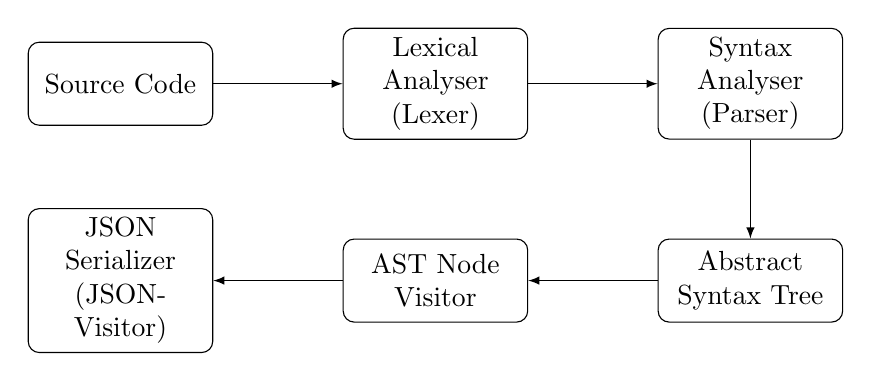
\begin{tikzpicture}[node distance=2cm, auto]
  % Define block styles
  \tikzstyle{block} = [rectangle, draw, text width=6em, text centered, rounded corners, minimum height=3em]
  \tikzstyle{line} = [draw, -latex]
  
  % Place blocks
  \node [block] (source) {Source Code};
  \node [block, right of=source, node distance=4cm] (lexer) {Lexical Analyser (Lexer)};
  \node [block, right of=lexer, node distance=4cm] (parser) {Syntax Analyser (Parser)};
  \node [block, below of=parser, node distance=2.5cm] (ast) {Abstract Syntax Tree};
  \node [block, left of=ast, node distance=4cm] (visitor) {AST Node Visitor};
  \node [block, left of=visitor, node distance=4cm] (json) {JSON Serializer (JSONVisitor)};
  
  % Draw lines
  \path [line] (source) -- (lexer);
  \path [line] (lexer) -- (parser);
  \path [line] (parser) -- (ast);
  \path [line] (ast) -- (visitor);
  \path [line] (visitor) -- (json);
\end{tikzpicture}
\caption{High-level architecture of the \texttt{tinyC} compiler frontend}
\label{fig:architecture}
\end{figure}

The architecture consists of the following main components:

\begin{enumerate}
    \item \textbf{Lexical Analyser (Lexer)}: The lexer reads the source code character by character and groups them into tokens according to the lexical rules of \texttt{tinyC}. It handles whitespace, comments, and reports lexical errors.

    \item \textbf{Syntax Analyser (Parser)}: The parser takes the token stream produced by the lexer and verifies that it conforms to the \texttt{tinyC} grammar. It constructs an abstract syntax tree and reports syntax errors.

    \item \textbf{Abstract Syntax Tree (AST)}: The AST represents the hierarchical structure of the parsed program. Each node in the tree corresponds to a language construct in the source code.

    \item \textbf{AST Node Visitor}: The visitor pattern is used to traverse the AST for serialization.

    \item \textbf{JSON Serializer}: This component converts the AST to a JSON representation following a well-defined schema available in Appendix B.
\end{enumerate}

The core implementation is structured as a library (lib\texttt{tinyC}) that can be used directly in C++ projects. A separate command-line interface (\texttt{tinyC}-compiler) is built on top of this library, providing the standalone executable functionality.

\section{AST Design}

The AST design follows object-oriented principles to create a clear, maintainable, and extensible representation of \texttt{tinyC} programs.

\subsection{Node Structure}

The AST consists of various node types that represent different language constructs in \texttt{tinyC}. Each node contains specific fields relevant to its language construct and provides methods to access these fields. The design prioritizes simplicity for JSON parsing, allowing students to easily work with the AST representation regardless of their implementation language.

Key node categories include:

\begin{itemize}
    \item \textbf{Declaration Nodes}: Represent variable, function, and struct declarations
    \item \textbf{Type Nodes}: Represent primitive types, named types, and pointer types
    \item \textbf{Expression Nodes}: Represent literals, identifiers, binary and unary operations, etc.
    \item \textbf{Statement Nodes}: Represent blocks, conditionals, loops, etc.
\end{itemize}

\subsection{Memory Management}

The AST uses \texttt{std::unique\_ptr} for managing node ownership, ensuring that:
\begin{enumerate}
    \item Memory is automatically managed, preventing leaks
    \item Ownership semantics are clear: each node can have only one owner
    \item There is no overhead compared to raw pointers
\end{enumerate}

This approach aligns with modern C++ best practices and provides a good balance between safety and performance.

\subsection{Visitor Pattern Implementation}

The visitor pattern is implemented to allow operations on the AST without modifying the node classes. The base \texttt{NodeVisitor} interface declares virtual \texttt{visit} methods for each concrete node type, as shown in Listing~\ref{code:node-visitor-interface}:

\begin{listing}[ht!]
\begin{verbatim}
class NodeVisitor {
public:
    virtual ~NodeVisitor() = default;
    
    // Visit methods for declaration nodes
    virtual void visit(const VariableNode& node) = 0;
    virtual void visit(const FunctionDeclarationNode& node) = 0;
    // ... other declarations
    
    // Visit methods for type nodes
    virtual void visit(const PrimitiveTypeNode& node) = 0;
    // ... other types
    
    // Visit methods for expression nodes
    virtual void visit(const LiteralNode& node) = 0;
    // ... other expressions
    
    // Visit methods for statement nodes
    virtual void visit(const BlockStatementNode& node) = 0;
    // ... other statements
};
\end{verbatim}
\caption{NodeVisitor interface declaration}
\label{code:node-visitor-interface}
\end{listing}

Each AST node implements an \texttt{accept} method that invokes the appropriate \texttt{visit} method on the visitor, as demonstrated in Listing~\ref{code:block-stmt-node-accept}:

\begin{listing}[ht!]
\begin{verbatim}
void BlockStatementNode::accept(NodeVisitor& visitor) const {
    visitor.visit(*this);
}
\end{verbatim}
\caption{BlockStatementNode's accept method}
\label{code:block-stmt-node-accept}
\end{listing}

This design allows for adding new operations on the AST without modifying the node classes, adhering to the Open-Closed Principle as discussed in the visitor pattern implementation.


\subsection{Source Location Tracking}

Each AST node includes source location information to facilitate error reporting and debugging, as shown in Listing~\ref{code:ast-node-base-class}:

\begin{listing}[ht!]
\begin{verbatim}
class ASTNode {
public:
    explicit ASTNode(lexer::SourceLocation location);
    virtual ~ASTNode() = default;
    
    [[nodiscard]] lexer::SourceLocation getLocation() const;
    
    virtual void accept(NodeVisitor& visitor) const = 0;

private:
    const lexer::SourceLocation location;
};
\end{verbatim}
\caption{ASTNode base class declaration}
\label{code:ast-node-base-class}
\end{listing}

The \texttt{SourceLocation} struct contains:
\begin{itemize}
    \item The filename
    \item The line number (1-based)
    \item The column number (1-based)
\end{itemize}

This information is preserved throughout the compilation process and included in the JSON output, as we'll see in Section 5.3.

\section{API Design}

The \texttt{tinyC} compiler frontend provides two main interfaces: a C++ library API and a command-line interface.

\subsection{Library API}

The library API allows direct integration of the \texttt{tinyC} frontend into C++ projects. The main entry points are:

\begin{enumerate}
    \item \textbf{Lexer Class}: For tokenizing source code, as shown in Listing~\ref{code:lexer-interface}:
\begin{listing}[ht!]
\begin{verbatim}
namespace tinyC::lexer {
    class Lexer {
    public:
        explicit Lexer(std::string source, std::string filename = "<input>");
        TokenPtr nextToken();
        std::vector<TokenPtr> tokenize();
    };
}
\end{verbatim}
\caption{Lexer class interface}
\label{code:lexer-interface}
\end{listing}

    \item \textbf{Parser Class}: For parsing tokens into an AST, as shown in Listing~\ref{code:parser-interface}:
\begin{listing}[ht!]
\begin{verbatim}
namespace tinyC::parser {
    class Parser {
    public:
        explicit Parser(lexer::Lexer& lexer);
        ast::ASTNodePtr parseProgram();
    };
}
\end{verbatim}
\caption{Parser class interface}
\label{code:parser-interface}
\end{listing}

    \item \textbf{Visitor Classes}: For traversing and operating on the AST, as shown in Listing~\ref{code:visitor-classes}:
\begin{listing}[ht!]
\begin{verbatim}
namespace tinyC::ast {
    class DumpVisitor : public NodeVisitor {
    public:
        explicit DumpVisitor(std::ostream& os);
        // Visit methods for all node types
    };
    
    class JSONVisitor : public NodeVisitor {
    public:
        explicit JSONVisitor(bool prettyPrint = true);
        std::string getJSON() const;
        // Visit methods for all node types
    };
}
\end{verbatim}
\caption{Visitor classes for AST traversal}
\label{code:visitor-classes}
\end{listing}
\end{enumerate}

This API design allows for flexible use of the frontend, enabling students to:
\begin{itemize}
    \item Directly work with the AST classes in their backend implementations
    \item Implement their own visitors for custom AST operations
    \item Control the parsing process step by step
\end{itemize}

\subsection{Command-Line Interface}

The command-line interface provides a standalone executable for parsing \texttt{tinyC} source files and outputting the AST as JSON. The main functionalities include:

\begin{enumerate}
    \item \textbf{Lexical Analysis Mode}, as shown in Listing~\ref{code:lex-mode-command}:
\begin{listing}[h]
\begin{verbatim}
tinyC-compiler --lex file.tc
\end{verbatim}
\caption{Lexical analysis mode command}
\label{code:lex-mode-command}
\end{listing}
    This mode tokenizes the input file and outputs the tokens.

    \item \textbf{Parsing Mode}, as shown in Listing~\ref{code:parse-mode-command}:
\begin{listing}[h]
\begin{verbatim}
tinyC-compiler --parse file.tc
\end{verbatim}
\caption{Parsing mode command}
\label{code:parse-mode-command}
\end{listing}
    This mode parses the input file and outputs the AST as JSON.

    \item \textbf{Interactive Mode}, as shown in Listing~\ref{code:interactive-mode-command}:
\begin{listing}[h]
\begin{verbatim}
tinyC-compiler
\end{verbatim}
\caption{Interactive mode command}
\label{code:interactive-mode-command}
\end{listing}
    This mode provides an interactive shell for entering \texttt{tinyC} code and seeing the resulting tokens or AST.
\end{enumerate}

The command-line interface is designed to be simple and intuitive, with clear error messages and help text, making it accessible to students with varying levels of experience.

\subsection{JSON Output Format}

The JSON output format provides a standardized representation of the AST that can be consumed by any programming language. The format follows a well-defined schema with the following key characteristics:

\begin{enumerate}
    \item \textbf{Node Type Identification}: Each node includes a \texttt{nodeType} field that identifies its type.
    \item \textbf{Hierarchical Structure}: The JSON structure mirrors the hierarchical structure of the AST.
    \item \textbf{Source Locations}: Each node includes location information with filename, line, and column.
    \item \textbf{Type-Specific Fields}: Each node type includes fields specific to that language construct.
\end{enumerate}

Example JSON output for a simple variable declaration is shown in Listing~\ref{code:json-example}:
\begin{listing}[h!]
\begin{verbatim}
{
  "nodeType": "Program",
  "declarations": [
    {
      "nodeType": "VariableDeclaration",
      "identifier": "x",
      "type": {
        "nodeType": "PrimitiveType",
        "kind": "int",
        "location": {
          "filename": "example.tc",
          "line": 1,
          "column": 1
        }
      },
      "initializer": {
        "nodeType": "Literal",
        "kind": "integer",
        "value": "42",
        "location": {
          "filename": "example.tc",
          "line": 1,
          "column": 7
        }
      },
      "location": {
        "filename": "example.tc",
        "line": 1,
        "column": 5
      }
    }
  ],
  "location": {
    "filename": "example.tc",
    "line": 1,
    "column": 1
  }
}
\end{verbatim}
\caption{Example JSON output for a variable declaration}
\label{code:json-example}
\end{listing}

The complete JSON schema is provided in Appendix B, which defines the structure for all node types supported by the frontend.

\pagebreak

\section{Test Suite Architecture}
The test suite for the TinyC compiler frontend is a comprehensive framework designed to validate the correctness of both the provided implementation and student-created alternatives. It offers systematic verification of lexical analysis, parsing functionality, and error handling capabilities.
\subsection{Test File Structure and Format}
The test files follow a metadata-driven format that allows precise specification of expected outcomes. Each test file contains:
\begin{enumerate}
\item \textbf{Standardized Header Metadata:}
\begin{itemize}
\item \texttt{// tinyC TEST} marker indicating a test file
\item \texttt{// INFO:} description of the test's purpose
\item \texttt{// RUN:} test type specification (parser, exec)
\item \texttt{// EXPECT:} expected outcome (SUCCESS, PARSER_ERROR, \\or LEXER_ERROR)
\item \texttt{// RESULT:} expected JSON output (for SUCCESS tests only)
\end{itemize}
\item Actual TinyC code following the metadata section
\end{enumerate}
This approach separates test expectations from the code being tested, making it easier to understand the purpose of each test and to verify correct functionality. The addition of the \texttt{RUN} directive enables the test framework to support different testing modes, particularly distinguishing between parser validation tests and execution tests that can be used once a backend implementation is available.

\subsection{Test Categories}


The test suite encompasses several categories of tests. The basic language feature tests cover empty programs, variable declarations and initializations, arrays and pointers, basic expressions and operations, and function declarations and definitions. Advanced language feature tests include control structures (if-else, loops, switch-case), struct declarations and usage, function pointers, type casting, and complex expressions with nested operations.

For error handling, the test suite verifies proper detection and reporting of lexical errors (such as invalid characters and unterminated strings/comments) and syntax errors (including mismatched parentheses and missing semicolons). Additionally, the test suite addresses edge cases by testing deeply nested expressions, complex combinations of language features, and boundary conditions for different constructs.

These comprehensive test categories ensure that the parser correctly handles the full spectrum of TinyC language features while providing appropriate error messages for invalid inputs.

\subsection{Test Runner Capabilities}
The \texttt{test_runner.py} script provides sophisticated test execution and validation:
\subsubsection*{Flexible Test Selection}
The runner supports targeted testing through:
\begin{itemize}
\item Running individual tests by number (\texttt{--test} flag)
\item Running a range of tests (\texttt{--range} flag)
\item Running all available tests by default
\end{itemize}
\subsubsection*{Robust Output Validation}
For successful parses, the runner performs:
\begin{itemize}
\item JSON schema validation against a formal specification
\item Structural comparison between expected and actual AST structures
\item Smart comparison that focuses on semantic equivalence rather than exact string matching
\item Proper handling of source location information (which can vary but must follow the correct format)
\end{itemize}
\subsubsection*{Error Detection Validation}
For error tests, the runner:
\begin{itemize}
\item Verifies that the appropriate error type is reported (lexical or syntax)
\item Checks for informative error messages
\item Validates that the parser exits with a non-zero code for errors
\end{itemize}
\subsubsection*{Detailed Reporting}
The test runner provides:
\begin{itemize}
\item Clear test-by-test reports showing pass/fail status
\item Detailed error diagnostics for failed tests
\item Comparison of expected vs. actual outputs with previews
\item Aggregated summary statistics at the end
\end{itemize}
\subsection{Schema Validation}
The test suite includes a formal JSON schema that defines the expected structure of the AST:
\begin{itemize}
\item Validates node types and required fields
\item Ensures proper nesting of AST components
\item Verifies that source location information is present and properly formatted
\end{itemize}
The schema serves both as documentation of the JSON format and as a validation tool, ensuring that AST outputs conform to the expected structure. This is particularly valuable for students implementing their own parsers, as it provides immediate feedback about structural correctness.
% \begin{listing}[ht]
% \begin{minted}{json}
% {
%     "type": "object",
%     "properties": {
%         "nodeType": {
%         "enum": ["Program"]
%     },
%     "declarations": {
%         "type": "array",
%         "items": {
%             "oneOf": [
%                 { "$ref": "#/definitions/VariableDeclaration" },
%                 { "$ref": "#/definitions/FunctionDeclaration" },
%                 { "$ref": "#/definitions/StructDeclaration" },
%                 { "$ref": "#/definitions/FunctionPointerDeclaration" }
%             ]
%         }
%     },
%     "location": { "$ref": "#/definitions/SourceLocation" }
%     },
%     "required": ["nodeType", "declarations", "location"]
% }
% \end{minted}
% \caption{Excerpt from the JSON schema showing the root Program node structure}
% \label{code}
% \end{listing}
\subsection{Test Generation Utilities}
The \texttt{test_generator.py} utility complements the test runner by:
\begin{itemize}
\item Automatically generating test files from example TinyC code
\item Creating expected JSON outputs for validation
\item Maintaining a consistent test nomenclature and organization
\item Supporting different test categories with appropriate descriptions
\end{itemize}
The test generator provides a systematic way to create new tests as the implementation evolves, ensuring consistent test coverage across language features.
\subsection{Educational Value}
The test suite is designed with educational objectives in mind:
\begin{itemize}
\item Tests progressively introduce language features, helping students understand the language incrementally
\item Detailed error reporting guides students toward correct implementations
\item The test framework itself demonstrates good testing practices
\item Students can extend the test suite with their own tests as they implement additional features
\end{itemize}




\section{Summary}

This chapter has outlined the design requirements and architecture of the \texttt{tinyC} compiler frontend. The functional and non-functional requirements define what the system must accomplish and how it should behave. The \texttt{tinyC} grammar analysis identified key challenges and informed the parsing approach. The system architecture, AST design, API specifications, and test suite architecture collectively provide a comprehensive blueprint for an educational compiler frontend that meets the needs of NI-GEN course students.

The design emphasizes clarity, modularity, and educational value, enabling students to focus on compiler middle-end and back-end development while providing a solid foundation for understanding compiler frontends.